\documentclass[3p]{elsarticle} %preprint/3p

\usepackage{hyperref}

\journal{ }

\usepackage{amsmath} %added for maths environments (equation and align)
\usepackage{amssymb}
\usepackage{bm} %bold symbols by using \bm
\usepackage{mathtools} %added for \xrightleftharpoons

\usepackage{subcaption} %allowing for subcaptions and subfigures
\captionsetup[sub]{font=normalsize}%normalsize

\usepackage[autostyle]{csquotes}
\MakeOuterQuote{"}

\biboptions{sort&compress}
\bibliographystyle{elsarticle-num}

% slightly altering rules for figure placement to prevent full-page figures
\usepackage{placeins}
\renewcommand{\floatpagefraction}{.90}
\renewcommand{\topfraction}{.90}

\usepackage[capitalise]{cleveref}

\usepackage{todonotes} %added for todo notes
\let\oldtodo\todo
\renewcommand{\todo}[1]{\oldtodo[inline]{#1}}
%\renewcommand{\todo}[1]{\oldtodo[color=white!40,inline]{#1}}
\newcommand{\toask}[1]{\oldtodo[color=green!40, inline]{#1}}
\newcommand{\wrn}[1]{\oldtodo[color=red!40, inline]{#1}}

\usepackage{xcolor}
\usepackage{listings}
\usepackage{lstautogobble}
\usepackage[numbered]{matlab-prettifier}
\lstdefinestyle{mystyle}{
	numbers=left,
	numberstyle=\footnotesize,
	numbersep=8pt,
	style=Matlab-editor,
	tabsize=4,
	basicstyle=\ttfamily\footnotesize,
	numbersep=25pt,
	frame=none,
	autogobble=true
}

\newcommand{\citeMe}{\href{https://doi.org/10.1016/j.electacta.2023.142624}{T. Hageman \& C. Andrade \& E. Martínez-Pañeda, Corrosion rates under charge-conservation conditions. Electrochimica Acta 461 (2023) 142624} \citep{Hageman2023}}

\begin{document}

\begin{frontmatter}
\title{Corr\textunderscore Sup\textunderscore Surf\textunderscore Sim: a MATLAB code to analyse corrosion rates under charge conservation conditions.}

\author[1]{Tim Hageman \corref{mycorrespondingauthor}}
\cortext[mycorrespondingauthor]{Corresponding author}
\ead{t.hageman@imperial.ac.uk}
\author[1]{Emilio Martínez-Pañeda}
\author[2]{Carmen Andrade}

\address[1]{Department of Civil and Environmental Engineering, Imperial College London, London SW7 2AZ, UK}
\address[2]{International Center of Numerical Methods in Engineering (CIMNE), Madrid 28010, Spain}

\begin{abstract}
\begin{center}
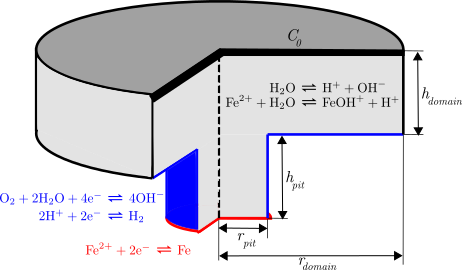
\includegraphics[width=12cm]{../Figures/Domain.png}
\end{center}
Documentation that accompanies the \textit{MATLAB} code \href{https://github.com/T-Hageman/Corr_Sup_Surf_Sim}{Corr\textunderscore Sup\textunderscore Surf\textunderscore Sim (available here)}, which enables the simulation of natural corrosion under charge conservation conditions. This documentation explains the usage of the implemented finite element framework, and highlight the main files. If using this module for research or industrial purposes, please cite: \citeMe{}.
\end{abstract}

\begin{keyword}
MATLAB, electrochemistry, finite element method, charge conservation, corrosion
\end{keyword}

\end{frontmatter}

\tableofcontents

\section{Introduction}
While localised corrosion is responsible for many catastrophic failures, the corrosion process itself is difficult to predict \citep{Galvele1976}. Both lab experiments and numerical simulations commonly prescribe the electric potential of the metal, to accelerate experimental procedures or match simulation to experiments \citep{Gravano1984, Sun2021, Laycock2001, Mai2016, Nguyen2022, Li2020}. However, for most cases of natural corrosion no potential is prescribed, instead requiring the corroding metal to be self-sufficient. This "self-sufficiency" requires the electrons produced by anodic corrosion reaction to be directly consumed by counteracting cathodic reactions. The simulation framework presented here, and described in \citep{Hageman2023}, enables corrosion simulation under these self-sufficiency conditions by dynamically resolving the metal potential to balance the cathodic and anodic currents. 

\subsection{Basic usage}
For simulating the model as provided, running the function "main.m" performs all required actions: It automatically generates the geometry and mesh, initialises all simulation components, and prints outputs to the screen and saves them to a folder within results. Simple changes, e.g. editing geometric and reaction parameters, can be done within main.m without requiring altering other files. 

\section{Summary of included files}
The code is set up in a object-oriented manner, defining matlab classes for each sub-component and providing their accompanying methods. As a result, a clear distinction is made between different components, and each can be used and altered with limited/no impact on other components. Here, the different classes are described. The commenting style employed within the code is compatible with the matlab help function, as such information about all usable methods within a class can be accessed by including the relevant folders, and typing, for instance, "help Solver" to print all variables contained within and all function available from the solver. 

\subsection{main.m}
This is the main file, from which all classes are constructed and the actual simulation is performed. Within it, all properties used within other classes are defined as inputs, for instance for the description of the electrolyte:
\lstinputlisting[firstnumber=75,firstline=75,lastline=84,style=mystyle,title=main.m]{../main.m}
where "physics{\_}in" is the array of options (in this case, physical models) passed to the physics object at construction. 

The actual time-dependent simulations are also performed within this file:
\lstinputlisting[firstnumber=169,firstline=169,lastline=177,style=mystyle,title=main.m]{../main.m}
\lstinputlisting[firstnumber=195,firstline=195,lastline=198,style=mystyle]{../main.m}
Notably, while this performs the time-stepping scheme and controls the time increment size and termination of the simulations, it does not by itself solve anything, instead calling the "solver.Solve()" function which performs a Newton-Raphson procedure using the parameters used to initialize the class, and once the current timestep is converged returns to the main code.

\subsection{Models}
The files included within the Models folder form the main implementation of all the physical phenomena involved. They implement the assembly of tangential matrices and force vectors, when requested by the solving procedures, and store model-specific parameters. 

\subsubsection{BaseModel}
This is an empty model, inherited by all other models to provide consistency within the available functions. While empty within here, the potential functions that can be defined within other models include assembling the system matrix and force vector:
\lstinputlisting[firstnumber=27,firstline=27,lastline=27,style=mystyle,title=Models/@BaseModel/BaseModel.m]{../Models/@BaseModel/BaseModel.m}
, and committing history dependent or path dependent variables:
\lstinputlisting[firstnumber=14,firstline=14,lastline=14,style=mystyle]{../Models/@BaseModel/BaseModel.m}
where the keyword "commit{\_}type" indicates the type of history or path dependence to commit at the current point. 

\subsubsection{Constrainer}
This model is used to apply fixed boundary constraints to a degree of freedom at a set location. Within the main file, the inputs required are:
\lstinputlisting[firstnumber=119,firstline=119,lastline=123,style=mystyle,title=main.m]{../main.m}
and multiple definitions of this model are allowed, allowing for constraints to be applied to several element groups. These constraints are integrated within the tangential matrix and force vector through  allocation matrices $\bm{C}_{con}$ and $\bm{C}_{uncon}$, reordering the system into a constrained and unconstrained part. This allows the constrained system to be solved as:
\begin{equation}
	\bm{C}_{uncon}^T \bm{K} \bm{C}_{uncon} \mathbf{y} = -\left(\bm{C}_{uncon}^T\bm{f}+\bm{C}_{uncon}^T \bm{K} \bm{C}_{con}\mathbf{c}\right)
\end{equation}
with the values of the boundary constraints contained in the vector $\mathbf{c}$. After solving, the state vector is then incremented through:
\begin{equation}
	\mathbf{x}^{new} = \mathbf{x}^{old} + \bm{C}_{uncon}\mathbf{y} + \bm{C}_{con}\mathbf{c}
\end{equation}

\subsubsection{OxygenLimiter}
Similar to the "constrainer" model detailed in the previous section, but also accepts a time up to which the constraints are applied. After this time is reached, no further constraints are applied by this model. Required input properties to be defined:
\lstinputlisting[firstnumber=105,firstline=105,lastline=111,style=mystyle,title=main.m]{../main.m}

\subsubsection{Electrolyte}
The electrolyte model implements the Nernst-Planck mass balance:
\begin{equation}
    \dot{C}_{\pi}+\bm{\nabla}\cdot\left(-D_\pi \bm{\nabla}C_\pi\right) + \frac{z_\pi F}{RT} \bm{\nabla} \cdot \left(-D_\pi C_\pi \bm{\nabla} \varphi\right) +R_\pi = 0 
\end{equation}
for the ionic species and their name within the model file: $\mathrm{H}^+$ ("H"), $\mathrm{OH}^-$ ("OH"), $\mathrm{Na}^+$ ("Na"), $\mathrm{Cl}^-$ ("Cl"), $\mathrm{Fe}^{2+}$ ("Fe"), and $\mathrm{FeOH}^{+}$ ("FeOH"). Additionally, it implements the electro-neutrality condition \citep{Feldberg2000, Sarkar2011}:
\begin{equation}
	\sum z_\pi C_\pi = 0
\end{equation}
and bulk reactions:
\begin{equation}
    \mathrm{H}_2\mathrm{O} \xrightleftharpoons[k_{w}']{k_{w}} \mathrm{H}^+ + \mathrm{OH}^- \label{react:water}
\end{equation}
\begin{equation}
    \mathrm{Fe}^{2+} + \mathrm{H}_2\mathrm{O} \xrightleftharpoons[k_{fe}']{k_{fe}} \mathrm{FeOH}^+ + \mathrm{H}^+ \label{react:fe_feoh}
\end{equation}
\begin{equation}
    \mathrm{FeOH}^{+} + \mathrm{H}_2\mathrm{O} \xrightharpoonup{k_{feoh}} \mathrm{Fe}(\mathrm{OH})_2 + \mathrm{H}^+ \label{react:feoh_feoh2}
\end{equation}
with reaction rates:
\begin{equation}
    R_{\mathrm{H}^+,w}=R_{\mathrm{OH}^-} = k_{w}C_{\mathrm{H}_2\mathrm{O}} - k_{w}'C_{\mathrm{H}^+}C_{\mathrm{OH}^-}  = k_{eq} \left(K_w-C_{\mathrm{H}^+} C_{\mathrm{OH}^-} \right) \label{eq:water_react}
\end{equation}
\begin{align}
    R_{\mathrm{Fe}^{2+}}&=-k_{fe}C_{\mathrm{Fe}^{2+}}+k_{fe}'C_{\mathrm{FeOH}^+}C_{\mathrm{H}^+} \\
    R_{\mathrm{FeOH}^+}&=k_{fe}C_{Fe^{2+}}-C_{\mathrm{FeOH}^+}(k_{feoh}+k_{fe}'C_{\mathrm{H}^+})\\
    R_{\mathrm{H}^+,fe}&=k_{fe}C_{\mathrm{Fe}^{2+}}-C_{\mathrm{FeOH}^+}(k_{fe}'C_{\mathrm{H}^+}-k_{feoh}) \label{eq:H_Part2}
\end{align}
For this model, the input properties required are:
\lstinputlisting[firstnumber=75,firstline=75,lastline=84,style=mystyle,title=main.m]{../main.m}
This model employs a lumped integration scheme when the vector "Lumped" contains true \citep{Hageman2023Lumped}.

\subsubsection{ElectrolyteInterface}
Finally, the electrolyteInterface model implements the metal-electrolyte coupling through the corrosion reaction at the anodic surface:
\begin{equation}
    \mathrm{Fe}^{2+}+2\mathrm{e}^-\xrightleftharpoons[k_{c}']{k_{c}}\mathrm{Fe}
\end{equation}
and the cathodic surface includes oxygen and hydrogen-related reactions:
\begin{align}
    \mathrm{O}_2+2\mathrm{H}_2\mathrm{O} +4\mathrm{e}^-\xrightleftharpoons[k_{o}']{k_{o}} 4 \mathrm{OH}^- \\
    2\mathrm{H}^+ + 2\mathrm{e}^-\xrightleftharpoons[k_{h}']{k_{h}} H_2 
\end{align}
It also implements the charge conservation at the surface:
\begin{equation}
    \int_\Gamma i_c+i_o+i_h\;\mathrm{d}\Gamma = \int_\Gamma 2F\nu_c + 4F\nu_o + 2F\nu_h \;\mathrm{d}\Gamma= 0
    \label{eq:current_conservation}
\end{equation}

For this model, the input variables to define are given as:
\lstinputlisting[firstnumber=86,firstline=86,lastline=97,style=mystyle,title=main.m]{../main.m}
with the vector "Lumped" allowing for individual interface reactions to be either integrated using a standard Gauss integration scheme (0) or a lumped integration scheme (1). the reaction constants matrix k is defined as:
\begin{equation}
	k = \begin{bmatrix} 
	k_{c} & k_{c}' & \alpha_{c} & E_{eq,c} \\ 
	k_{h} & k_{h}' & \alpha_{h} & E_{eq,h} \\ 
	k_{o} & k_{o}' & \alpha_{o} & E_{eq,o} \\ 
	\end{bmatrix}
\end{equation}

\subsection{Mesh}
This class contains the nodes and elements that describe the geometry, and provides support for evaluating shape functions. Within its implementation, it uses a multi-mesh approach, defining element groups for each entity within the domain (for instance, defining an element group "Electrolyte" for the electrolyte domain composed of surface elements, and defining an element group "Anode" composed of line elements which coincide with the anodic part of the metal-electrolyte boundary). The geometry of the problem is defined through procedures within the mesh class, specifically within "@Mesh/CorrosionPit{\_}Generator.m":
\lstinputlisting[firstnumber=27,firstline=27,lastline=30,style=mystyle,title=@Mesh/CorrosionPit{\_}Generator.m]{../@Mesh/CorrosionPit_Generator.m}
Defining rectangle R1 to represent the outer part of the domain and rectangle R2 for the pit. The mesh uses the standard matlab mesh generator "GenerateMesh" to convert this geometric description, allowing for element sizes to be defined:
\lstinputlisting[firstnumber=42,firstline=42,lastline=44,style=mystyle]{../@Mesh/CorrosionPit_Generator.m}
which allows for defining minimum element sizes through Hedge, and maximum sizes through Hmax. 

The mesh class also provides a direct interface from which to get the element shape functions, providing an element group number and the index of the element itself:
\lstinputlisting[firstnumber=20,firstline=20,lastline=21,style=mystyle,title=@Mesh/mesh.m]{../@Mesh/Mesh.m}
which returns a matrix containing the shape functions N within all integration points of the element, gradients of the shape function G, and the integration weights for all integration points w. 

\subsection{Shapes}
The classes within this folder provide basic shape functions, and are used by the mesh to provide shape functions and integration weights. The included shape functions are square Lagrangian and triangular Bernstein surface elements (Q9 and T6) and quadratic Lagrangian and Bernstein line elements (L3 and L3B).

\subsection{Physics}
This class provides all the support required for constructing and managing state and force vectors, tangential matrices, and boundary constraints. Most notably, during its initialization it generates an array of all the physical models, from which it then is able to construct the tangential matrix when required:
\lstinputlisting[firstnumber=48,firstline=48,lastline=63,style=mystyle,title=@Physics/Physics.m]{../@Physics/Physics.m}
This calls each of the models, and passes a handle to the physics object itself through which the individual models can add their contributions. 

The physics class also provides the ability for post-processing the results through the function;
\lstinputlisting[firstnumber=25,firstline=25,lastline=25,style=mystyle,title=@Physics/Physics.m]{../@Physics/Physics.m}
This function requires the name of a degree of freedom (for instance "H" for the hydrogen ion concentration), a scale to indicate whether the mesh is plotted in deformed (scale$>$0) or undeformed (scale$=$0) configuration (for the simulations performed, this is always $0$, since no solid deformations are simulated), and the name of an element group on which to plot the results ("Electrolyte", and "Anode"/"Cathode" for the metal-electrolyte interface.

\subsection{Dofspace}
This class converts the node numbering and degree of freedom type to an index for the degree of freedom, corresponding to its location within the unconstrained state vector and tangential matrix. Specific types of degree of freedom are registered through a string indicating their name:
\lstinputlisting[firstnumber=24,firstline=24,lastline=24,style=mystyle,title=@DofSpace/DofSpace.m]{../@DofSpace/DofSpace.m}
after which they can be added to nodes through:
\lstinputlisting[firstnumber=50,firstline=50,lastline=50,style=mystyle]{../@DofSpace/DofSpace.m}
These functions automatically check for duplicates, such that each model can safely add all the degrees of freedom relevant to itself, without taking into account potential interactions with other models. During the finite element assembly, the managed degrees of freedom indices are requestable by providing the degree of freedom type index and the node number:
\lstinputlisting[firstnumber=82,firstline=82,lastline=82,style=mystyle]{../@DofSpace/DofSpace.m}

\subsection{Solver}
The solver class implements a Newton-Raphson type nonlinear solver, including the ability to perform linear line-searches to improve the convergence rate and stability. During its creation, it gets linked to the physics object, such that it can automatically request updated tangential matrices. To obtain a solution for the linearised system, a sparse iterative solver is used (with as back-up option a direct solver) in conjunction with a preconditioner:
\lstinputlisting[firstnumber=21,firstline=21,lastline=43,style=mystyle,title=@Solver/Solve.m]{../@Solver/Solve.m}
in which the equilibriate preconditioner greatly decreases the conditioning number of the matrix, thereby reducing errors during the solving process. 

\section{Sample results}
Simulating the pencil electrode case as set up within "main.m" (equivalent to the case described in Sec. 4 from \citeMe{}, except for a smaller domain radius) automatically opens figures showing the results as the simulation proceeds. These results can also be obtained after it finishes. Results shown during the simulation are:
\lstinputlisting[firstnumber=284,firstline=284,lastline=284,style=mystyle,title=main.m]{../main.m}
\begin{center}
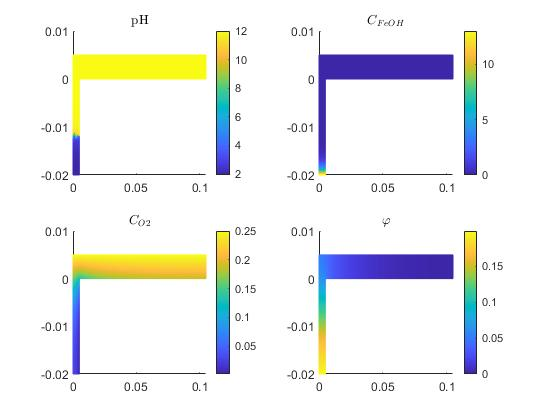
\includegraphics[width=12cm]{../Figures/Surfs.jpg}
\end{center}
which displays the pH, concentrations of $\mathrm{FeOH}^+$ ions and oxygen, and the electrolyte potential $\varphi$ at the current time (or, if done during post-processing, at the time the datafile was saved). Additionally, reaction rates can be obtained through
\lstinputlisting[firstnumber=279,firstline=279,lastline=279,style=mystyle,title=main.m]{../main.m}
\begin{center}
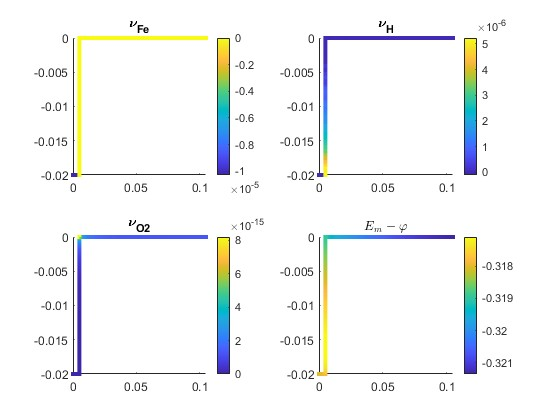
\includegraphics[width=12cm]{../Figures/Rates.jpg}
\end{center}
Showing the local reaction rates for the corrosion, hydrogen, and oxygen reactions, using the convention of possitive signs being electron-consuming, while negative signs indicate the electron-producing direction of the reactions. Additionally, the electric overpotential is shown at the interface.

Finally, temporal results are saved during the simulation via:
\lstinputlisting[firstnumber=179,firstline=179,lastline=185,style=mystyle,title=main.m]{../main.m}
which are then used to plot, for instance the reaction currents and matal potential via:
\lstinputlisting[firstnumber=261,firstline=261,lastline=274,style=mystyle,title=main.m]{../main.m}
\begin{center}
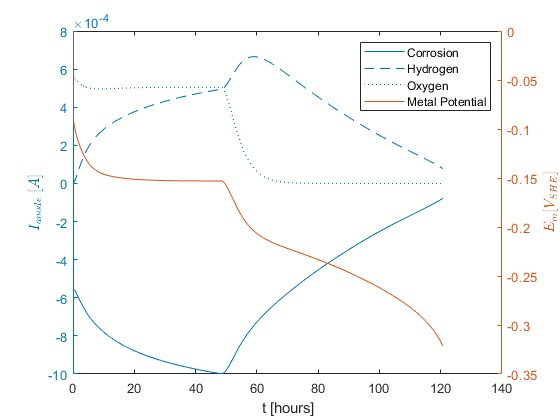
\includegraphics[width=12cm]{../Figures/Lines.jpg}
\end{center}

\bibliography{references}

\end{document}
